\documentclass{article}
\usepackage{amsmath}
\usepackage{amssymb}
\usepackage{graphicx}
\usepackage{hyperref}
\usepackage[version=4]{mhchem}


\begin{document}
(AMC) The sides \(P Q\) and \(P R\) of triangle \(P Q R\) are respectively of lengths 4 inches and 7 inches. The median \(P M\) is \(3 \frac{1}{2}\) inches. Then \(Q R\), in inches, is:\\
(A) 6\\
(B) 7\\
(C) 8\\
(D) 9\\
(E) 10\\
\centering
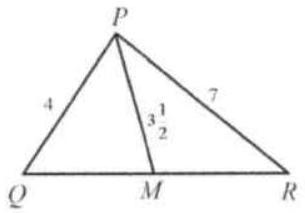
\includegraphics[width=\textwidth]{images/082.jpg}

Solution: (D).\\
Drop the perpendiculars \(P H\) at \(H\).\\
Let \(y\) denote half the length of \(Q R\), and let \(H M=x . M R=y\). Then \(Q H=y-x\).\\
Applying Pythagorean Theorem to \(\triangle Q P H, \triangle M P H\) :\\
\(4^{2}-(y-x)^{2}=\left(3 \frac{1}{2}\right)^{2}-x^{2}\)\\
Applying Pythagorean Theorem to \(\triangle Q P H, \triangle R P H\) :\\
\centering
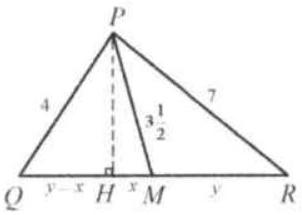
\includegraphics[width=\textwidth]{images/082(1).jpg}\\
\(4^{2}-(y-x)^{2}=(7)^{2}-(x+y)^{2}\)\\
From (1), we get \((y-x)^{2}-x^{2}=\frac{15}{4} \Rightarrow \quad y^{2}-2 x y=\frac{15}{4}\)


From (2), we get \((y+x)^{2}-(y-x)^{2}=33 \quad \Rightarrow \quad 4 x y=33\) (4) Solving the system of (3) and (4): \(y^{2}=\frac{33}{2}+\frac{15}{4}-\frac{81}{4} \quad \Rightarrow \quad y=\frac{9}{2}\). So \(Q R=9\).


\end{document}
